%--------------------------------------------------------------------------------------------------
\chapter{Stand der Technik}\label{cha:StandDerTechnik}

In diesem Kapitel gibt es einen Einblick in die drei Themenbereiche Industrie 4.0, industrielle Fertigung, Mensch-Computer Interaktion und Virtual Reality.
\newline\newline
Daher werden wir uns zunächst mit dem Begriff Industrie 4.0 auseinander setzen, den Begriff definieren und auf die Geschichte der Industriellen Revolutionen der vergangenen 260 Jahre sowie auf die Veränderungen in der Informations- und Kommunikationstechnik eingehen. Daraufhin gibt es einen Einblick in die Potentiale und Herausforderungen von Industrie 4.0. Zum Abschluss dieses Abschnittes wird ein Leitfaden zur Umsetzung von Industrie 4.0 für Unternehmen vorgestellt.
\newline\newline
Daraufhin gib es einen Einblick in die Ausgangslage der industriellen Fertigung, insbesondere in den Produktlebenszyklus, die Automatisierungspyramide und TODO...
\newline\newline
Als nächstes setzen wir uns auseinander mit dem Thema Mensch-Computer Interaktion (HCI). Dazu gibt es einen Einblick in die Geschichte der HCI der Vergangenen [XXX] Jahre, bevor wir aktuelle Entwicklungen in dem Bereich vorgestellt werden.
\newline\newline
Zum Schluss wird das Thema Virtual Reality (VR) vorgestellt und es gibt einen Einblick in die Geschichte, den Stand der Technik und technische Herausforderungen von Virtual Reality. Daraufhin werden vielversprechende Entwicklungen für die Zukunft von Virtual Reality vorgestellt.


%--------------------------------------------------------------------------------------------------
\section{Industrie 4.0}\label{sec:Industrie4.0}
Erstmalig tauchte der Begriff Industrie 4.0 auf der Hannover Messe 2011 auf und wurde daraufhin ein zentraler Bestandteil der Hightech-Strategie der deutschen Bundesregierung [8, BDI, Einblick i.d.4.Rev].
\newline
Der Begriff Industrie 4.0 „steht für die 4. Industrielle Revolution, einer neuen Stufe der Organisation und Steuerung der gesamten Wertschöpfungskette über den Lebenszyklus von Produkten“ [1, Anderl, Vortrag 2015]. Dies führt zum einem zu einer zunehmenden Vernetzung von „Mensch, Maschinen und Werkstücken durch Modernste Informations- und Kommunikationstechnik“ [6, BDI, Was ist Industrie 4.0], zum anderen auch zu einer zunehmenden „Vernetzung der realen mit der virtuellen Welt“ [7, DIN, Def. Ind.4]. Grundlage dieser Wandlung in der Industrie sind sogenannte Cyber-Physische-Systeme (CPS), also moderne Steuerungssysteme mit eingebetteten Softwaresystemen und Anbindung an das Internet (\cite{1}) [1, Anderl, Vortrag 2015]. Cyber-Physische-Systeme verknüpfen „reale (physische) Objekte und Prozesse mit informationsverarbeitenden (virtuellen) Objekten und Prozessen“ [11, Fraunhofer, CPS]. Die hat eine zunehmende Verschmelzung von Fertigungsprozessen und Informationstechnologie zur Folge [7, DIN, Def. Ind.4].

\subsection{Industrielle Revolution und Informations- und Kommunikationstechnik}\label{sec:GeschichteIndustrie4}

Um den Begriff Industrie 4.0 besser nachvollziehen zu können, ist es unumgänglich die Geschichte der industriellen Revolutionen der vergangenen 260 Jahre zu verstehen. Der Begriff Industrie 4.0 „leitet sich aus den großen Industriegeschichtlichen Umbrüchen ab“ [7, DIN, Def. Ind.4] und ist ein Wortspiel aus den Anteilen „Industrie“ und „4.0“. Der Anteil „4.0“ soll zum einem eine Assoziation zum Internet (Web 4.0) herstellen und zum anderen, wie in der heutigen Zeit üblich eine Versionsbezeichnung darstellen, wie man sie aus dem Bereich der Softwareentwicklung kennt [1, Anderl, Vortrag 2015].
\newline
Industrie 4.0 wird als „der vierte große Technologische Durchbruch“ [7, DIN, Def. Ind.4] betrachtet. Daher werden im Folgenden die industriellen Revolutionen bis zur Industrie 4.0 und die Entwicklung der Informations- und Kommunikationstechnik bis zu Web 4.0 betrachtet.

\subsubsection{Die industriellen Revolutionen}\label{sec:IndustrielleRevolution}
\begin{figure}[h]
	\centering
	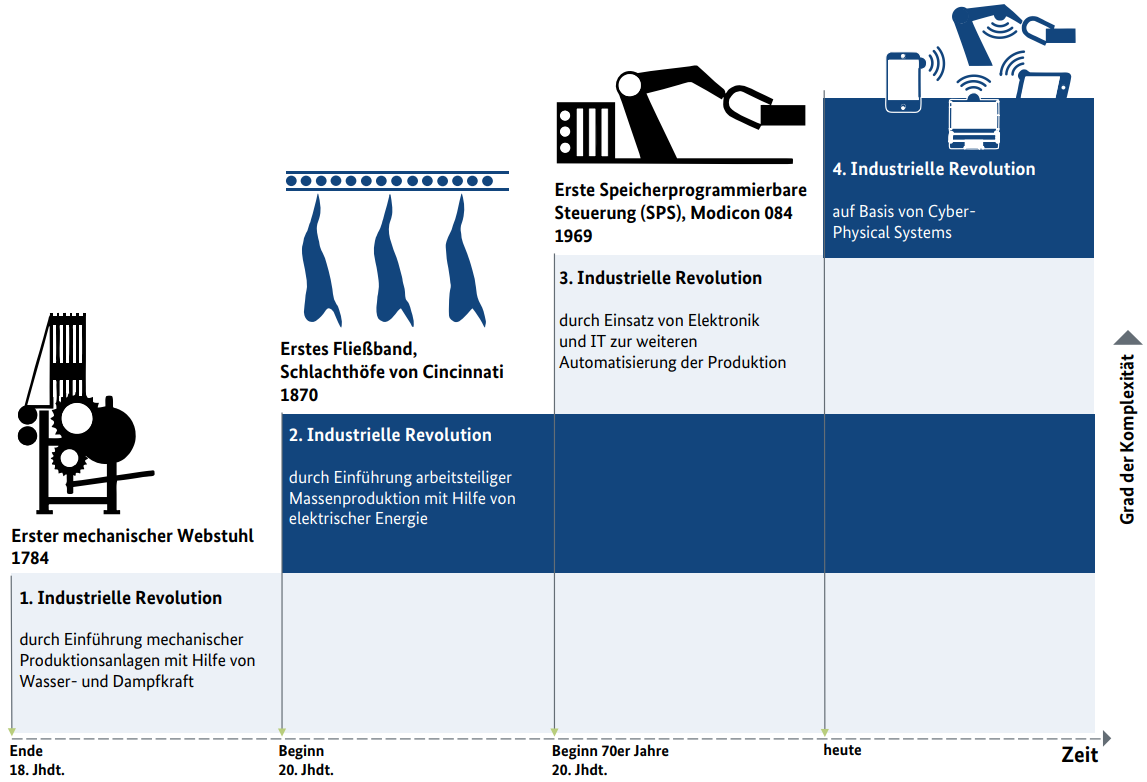
\includegraphics[width=1\linewidth]{Bilder/A1_DieGeschichteDerIndustriellenRevolutionenBMWI}
	\caption{Die Geschichte der Industriellen Revolutionen [A1, BMWi, S.8]}
	\label{fig:IndustrielleRevolutionenBild}
\end{figure}
\noindent Die \textbf{erste industrielle Revolution} spielte sich Mitte bis Ende des 18. Jahrhunderts ab. Im Fokus standen Wasser- und Dampfkraft, was die Möglichkeit mit sich brachte, Maschinen die vorher noch mit menschlicher Kraft angetrieben wurden, mithilfe von Wasser- und Dampfkraft anzutreiben. Die Menschen erkannten früh, dass sich durch die neuen industriellen Entwicklungen eine große Menge an Arbeitsplätzen schaffen lassen können. [9, Industrie Wegweiser, Ind.Wandel d.Z.]. Neben gesteigerter Produktivität in der Herstellung führte die erste industrielle Revolution dazu, „dass seit dieser Zeit in industriell geprägten Ländern keine strukturell bedingten Hungerkatastrophen mehr entstanden sind“ [B1, Bauernhansl, S.5]. Des Weiteren führte die verbesserte Infrastruktur durch Dampfschiffe und Eisenbahnen zu einer besseren Kleidungs- und Nahrungsversorgung und zu einem enormen Bevölkerungswachstum [B1, Bauernhansl, S.5]. Außerdem gab es große Auswirkungen auf die Gesellschaft, da zwei neue Schichten in der Bevölkerung entstanden: Die Fabrikarbeiterschaft und die Fabrikbesitzer. [B1, Bauernhansl, S.5]. Die Entwicklungen der ersten industriellen Revolution brachten allerdings einige große Probleme mit sich. Dazu gehören Beispielsweise die Ausbeutung der Fabrikmitarbeiter durch schlechte Arbeitsbedingungen und Bezahlung, Kinderarbeit und sogar eine verkürzte Lebenserwartung für die Fabrikmitarbeiter [B1, Bauernhansl, S.5].
\newline\newline
Die \textbf{zweite industrielle Revolution} zu Beginn des 20. Jahrhunderts „war geprägt durch Arbeitsteilige Massenproduktion mit Hilfe elektrischer Energie“ [B1, Bauernhansl, S.5]. Ermöglicht wurde die Massenproduktion unter anderem durch das von Henry Ford entwickelte Fließband, welches bereits 1913 in der Automobilproduktion eingesetzt wurde [10, Spiegel, Industrielle Revolutionen].Des Weiteren führten die Entwicklungen von elektrischen Antrieben und Verbrennungsmotoren zu einer zunehmenden Dezentralisierung. Dezentralisierung im Kontext der zweiten industriellen Revolution bedeutet, „die Arbeitsmaschinen nicht durch zentrale Kraftmaschinen anzutreiben, sondern dezentral zu betreiben“ [B1, Bauernhansl, S.5]. Ein weiterer „Erfolgsfaktor in der zweiten Industriellen Revolution waren die ersten Schritte der Globalisierung“ [9, Industrie Wegweise, I.i.W.d.Z.] durch die Fortschritte in der Verkehrsinfrastruktur. Dazu gehören Beispielsweise moderne Schiffe, die eine bessere Vernetzung zwischen den Kontinenten ermöglicht haben [9, Industrie Wegweise, I.i.W.d.Z.]. Für die Chemie- und Automobilindustrie wurde Erdöl zu einem wichtigen Rohstoff. „Die Großindustrielle Massenproduktion“ [B1, Bauernhansl, S.5] ermöglichte die Produktion von immer günstigeren (Konsum-)Gütern für die weiterhin wachsende Bevölkerung [B1, Bauernhansl, S.5]. Die Gesellschaft erkannte, dass die Ausbeutung der Fabrikarbeiter nicht weiter gehen kann und Gewerkschaften gewannen stark an Bedeutung. Daher sollten Fabrikarbeiter von nun an besser entlohnt werden, um weitere Soziale Spannungen zu vermeiden [B1, Bauernhansl, S.5]. Im Übergang zwischen der ersten und zweiten industriellen Revolution zum verbreiteten sich die Ideen des Kommunismus und der Sozialdemokratie [B1, Bauernhansl, S.5].
\newline\newline
Die \textbf{dritte industrielle Revolution} Mitte des 20. Jahrhunderts wurde geprägt zunehmende Automatisierung der Produktionsabläufe durch das einbinden von Elektronik und Informations- und Kommunikationstechnik [B1, Bauernhansl, S.7]. Durch den Einsatz von programmierbaren Steuerungen, „waren auch in den Fabriken Programmierer gefragt“ [10, Spiegel, Industrielle Revolutionen]. Des Weiteren wurde der Personal-Computer (PC) vermehrt im Büro aber auch im Haushalt eingesetzt [9, Industrie Wegweise, I.i.W.d.Z.]. Die Entwicklungen der dritten industriellen Revolution ermöglichten eine variantenreiche Serienproduktion. Mit dieser Entwicklung veränderten sich aber auch die Erwartungen der Kunden, welche nun vermehrt auf Individualität und Qualität der Produkte achteten [B1, Bauernhansl, S.7].
\newline\newline
Die \textbf{vierte industrielle Revolution} ist momentan noch im Gange. In Kapitel \ref{sec:PotentialeIndustrie4.0} und \ref{sec:HerausforderungenUmsetzung} gibt es einen Einblick in die Potentiale und Herausforderungen von Industrie 4.0. Vorweg lässt sich aber sagen, dass die vierte Industrielle Revolution die Industrie flexibler gestalten soll, statt ein höheres grad an Automatisierung zu erreichen. Die Wertschöpfung soll durch Cyber-Physische-Systeme verbessert werden. Es ist wichtig zu wissen, dass die Entwicklungen der Industrie 4.0 aus zwei Entwicklungsrichtungen kommen [1, Anderl, Vortrag 2015]:
\begin{enumerate}
	\item \textbf{Physicalize the Cyber} \\ Aus der Sicht der Informationstechnischen Unternehmen: „Zunehmende Nutzung von Informationstechnik in der Produktion“ [1, Anderl, Vortrag 2015].
	\item \textbf{Cyberize the Physical} \\ Aus der Sicht der Produktionstechnischen Unternehmen: „Anwendungen für Informationstechnik in der Produktion“ [1, Anderl, Vortrag 2015].
\end{enumerate}

\subsubsection{Informations- und Kommunikationstechnik}\label{sec:WebRevolution}
\begin{figure}[h]
	\centering
	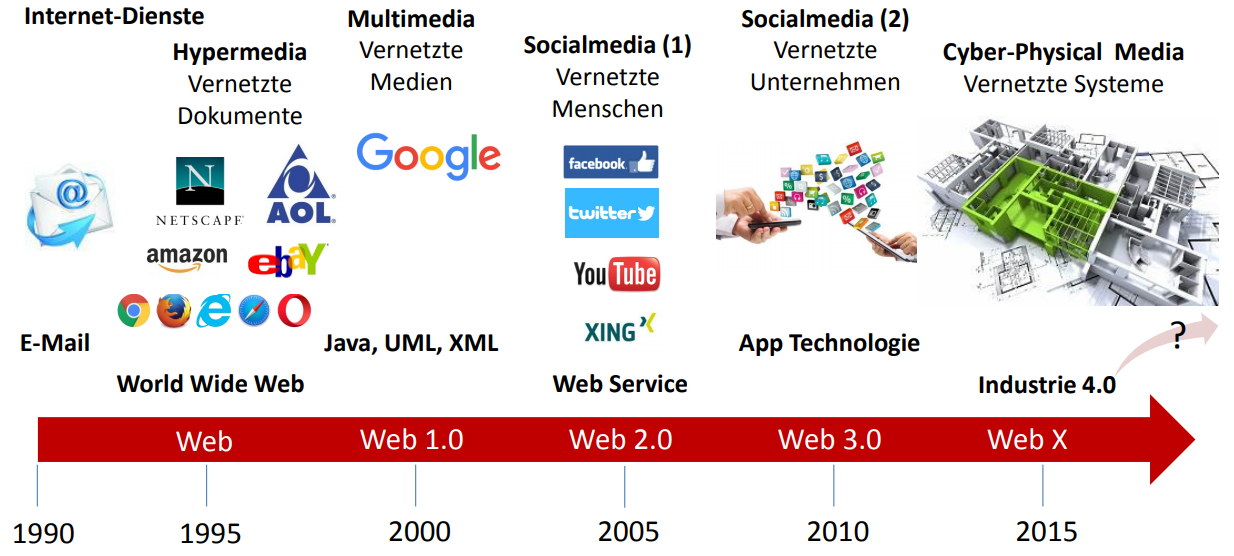
\includegraphics[width=1\linewidth]{Bilder/A2_EntwicklungWeb0-4}
	\caption{Die Entwicklung von Web bis Web 4.0 [A2, Kompet. Dig.Handwerk, S.3]}
	\label{fig:WebRevolutionBild}
\end{figure}
Genauso wie in der Industrie gab es in der Informations- und Kommunikationstechnik einige technologische Umbrüche. Auffällig ist, dass die sich die Technologien in der Informations- und Kommunikationstechnik im Vergleich zu den Fortschritten in der Industrie sehr schnell weiterentwickeln. Die wichtigsten Umbrüche sind in der Abbildung \ref{fig:WebRevolutionBild} zusammengefasst.
\newline\newline
Das wichtigste was man der Abbildung \ref{fig:WebRevolutionBild} entnehmen kann ist, dass in der neuen Entwicklungsstufe von Informations- und Kommunikationstechnik Cyber-Physische Medien im Mittelpunkt stehen.

\subsection{Potentiale von Industrie 4.0}\label{sec:PotentialeIndustrie4.0}

„Industrie 4.0 macht die Produktion individueller und effizienter“ [6, BDI, Was ist Industrie 4.0], ermöglicht durch das vernetzen von „Mensch, Maschinen und Werkstücken durch modernste Informations- und Kommunikationstechnik“ [6, BDI, Was ist Industrie 4.0]. Dies verspricht dem Wirtschaftsstandort Deutschland Wachstumschancen und sogar Wettbewerbsvorteile bei entsprechender Umsetzung. Laut dem Bundesverband der Deutschen Industrie (BDI) prognostizieren Experten eine Produktivitätssteigerung von bis zu 30 Prozent bis zum Jahr 2025 [6, BDI, Was ist Industrie 4.0].
\newline
Mit Industrie 4.0 sollen nicht nur große Unternehmen, sondern gezielt auch der Mittelstand angesprochen werden, um ihm wirtschaftlichen Nutzen bringen, da dieser das Rückgrat der deutschen Industrie bildet. Laut einer Studie der Commerzbank haben 86 Prozent der Unternehmen die Potentiale von Industrie 4.0 erkannt, zögern aber noch mit der Einführung [2, VDMA, Leitfaden, S.4]. Man kann sogar sagen, dass sich dem deutschen Mittelstand durch neuartige und innovative Produkte die Möglichkeit eröffnet, den Wandel zu Industrie 4.0 aktiv mitzugestalten [2, VDMA, Leitfaden, S.8]. Dennoch gibt es viele Unternehmen, denen „der konkrete Nutzen von Lösungsansätzen im Umfeld von Industrie 4.0 nicht ersichtlich“ ist [2, VDMA, Leitfaden, S.7]. 
\newline
Der Bundesverband der Deutschen Industrie e.V. hat die Unternehmensberatung Roland Berger mit einer „Studie zur digitalen Transformation der Industrie“ [8, BDI] beauftragt [8, BDI]. Die Studie kam zu dem Ergebnis, dass beim Verpassen der aktuellen Entwicklungen dem Wirtschaftsstandort Deutschland „Einbußen bei der industriellen Wertschöpfung bis 2025 von insgesamt 220 Milliarden Euro“ [8, BDI] drohen [8, BDI]. Europaweit rechnet man sogar mit Einbußen von bis zu 605 Milliarden Euro. Bei einem erfolgreichen Anknüpfen an den Wandel zu Industrie 4.0 „prophezeit die Studie der Automobilindustrie schon im Jahr 2025 ein sattes Wertschöpfungsplus von 35 Milliarden Euro“ [8, BDI] und dem Maschinen- und Anlagebau sogar bis zu 89 Milliarden Euro pro Jahr. Die Studie der Unternehmensberatung Roland Berger kam weiterhin zu dem Ergebnis, dass sich bereits 55 Prozent der befragten Unternehmen „bereits intensiv mit der Digitalen Transformation“ [8, BDI] beschäftigt haben, aber 43 Prozent die Bedeutung der Digitalisierung und des Wandels hauptsächlich in der Kostenreduktion sieht [8, BDI]. Des Weiteren schätzen sich rund ein Drittel der Unternehmen als hoch oder sehr hoch Digitalisiert ein, bei profitablen Unternehmen waren es sogar 62 Prozent.
\newline\newline
Im Folgenden sind vielversprechende Potentiale von Industrie 4.0 zusammengefasst:

\begin{enumerate}
	\item \textbf{Individualisierung der Kundenwünsche} [12, BMBF, Umsetz., S.19] \\
	Ermöglicht Rücksicht auf Individuelle Kundenwünsche zu nehmen. Dabei bleibt die 
	Produktion selbst bei Bestellungen von Einzelstücken oder Kleinstmengen (Losgröße 1) 
	effizient und rentabel [12, BMBF, Umsetz., S.19].
	
	\item \textbf{Flexibilisierung} [12, BMBF, Umsetz., S.20] \\
	Optimierungen „in unterschiedlichen Dimensionen: Qualität, Zeit, Risiko, Robustheit, Preis,
	Umweltverträglichkeit, etc.“ ermöglicht es die Produktionsprozesse flexibel zu gestalten,
	kurzfristig zu verändern und auf unerwartete Ausfälle zu reagieren [12, BMBF, Umsetz., S.20].
	
	\item \textbf{Optimierte Entscheidungsfindung} [12, BMBF, Umsetz., S.20] \\
	Durch das Sammeln von produktionstechnischrelevanten Daten in Echtzeit fällt es leichter
	die (richtigen) Entscheidungen zu treffen, um auf Störungen zu reagieren, 
	„standortübergreifende globale Optimierungen“ durchzuführen und auf dem globalen Markt 
	Wettbewerbsfähig zu bleiben [12, BMBF, Umsetz., S.20]. Daher sollte die Vernetzung der 
	Unternehmen nicht nur firmenintern und lokal, sondern auch Unternehmens übergreifend 
	(z.B. mit Zulieferern/Kunden) stattfinden [6, BDI, Was ist Ind4].

	\item \textbf{Ressourcenproduktivität und Effizienz} [12, BMBF, Umsetz., S.20] \\
	„Smart Factorys“, also Fabriken mit Produktionsanlagen die sich eigenständig und in Echtzeit 
	koordinieren und optimieren und somit die Produktion effizienter und flexibler gestalten [6, 
	BDI, Was ist Ind4]. Dabei wird bei gleichbleibendem oder sogar niedrigerem 
	Ressourceneinsatz die Produktionsmenge gesteigert [12, BMBF, Umsetz., S.20].

	\item \textbf{Wertschöpfungspotenziale durch neue Dienstleistungen} [12, BMBF, Umsetz., S.20] \\
	Es eröffnet sich ein neuer Markt für innovative Dienstleistungen, vorangetrieben durch die
	gesammelten Daten (Big Data) über den gesamten Lebenszyklus von intelligenten Produkten 
	[12, BMBF, Umsetz., S.20]. Durch das „Internet der Dinge“ (Internet of Things, kurz: IOT)
	werden intelligente Produkte zu Dienstleistungen, sogenannten „Smart Services“, da sie 
	während Ihrer gesamten Lebensdauert mit dem Internet verbunden sind [6, BDI, Was ist 
	Ind4].

	\item \textbf{Demografie-sensible Arbeitsgestaltung} [12, BMBF, Umsetz., S.20] \\
	Die Unternehmen bekommen durch verbesserte Arbeitsbedingungen die Chance auf den 
	demographischen Wandel zu reagieren und sogar davon profitieren zu können [12, BMBF, 
	Umsetz., S.20]. Durch den Fachkräftemangel und die alternde Bevölkerung ist es wichtig 
	„ältere Menschen länger in das Berufsleben einzubinden“ [6, BDI, Was ist Ind4].

	\item \textbf{Work-Life-Balance} [12, BMBF, Umsetz., S.20] \\
	Intelligente Assistenzsysteme helfen dabei, „den Arbeitseinsatz so zu gestalten, dass sowohl
	den Flexibilitätsbedürfnissen der Betriebe als auch den notwendigen Flexibilitätsspielräumen
	für den privaten Bereich in neuer Qualität Rechnung getragen werden kann“ [12, BMBF, 
	Umsetz., S.20]. Diese Assistenzsysteme können Unterschiedlich aussehen. Einige Beispiele
	dafür sind Mobile Geräte wie Tablet Computer oder Virtual/Augmented Reality Brillen [6, 
	BDI, Was ist Ind4].

	\item \textbf{Wettbewerbsfähigkeit als Hochlohnstandort} [12, BMBF, Umsetz., S.20] \\
	Deutschland gilt als ein Hochlohnstandort. Um auf den internationalen Markt 
	Wettbewerbsfähig zu sein müssen die Unternehmen genug Erwirtschaften um Profitabel
	zu sein [12, BMBF, Umsetz., S.20]. Industrie 4.0 gibt Unternehmen die Chance eine 
	Lohnenswerte Produktion im eigenen Land zu betreiben [12, BMBF, Umsetz., S.20].

	\item \textbf{Smart Products} [6, BDI, Was ist Ind4] \\
	Intelligente Produkte mit integrierten Chips (z.B. RFID Chips) liefern selbst alle benötigten
	Informationen für die Produktion. So kann Beispielweise ein Produkt einer Maschine 
	mitteilen, in welcher Farbe es lackiert werden soll. Des Weiteren liefern diese Chips Daten, 
	die für das virtuelle Abbild des Produktes und der Produktion genutzt werden. [6, BDI, Was 
	ist Ind4].

	\item \textbf{Simulation und Überwachung der Produktion} [6, BDI, Was ist Ind4] \\
	Durch einen digitalen Zwilling und die Sammlung von Daten in Echtzeit kann die gesamte
	Produktion simuliert und überwacht werden. Dies ermöglicht Beispielsweise die
	Fernsteuerung, Simulation und Überwachung der Produktion in Echtzeit[6, BDI, Was ist Ind4].

	\item \textbf{Chancen für IT-Unternehmen} [2, VDMA, Leitf., S.7] \\
	Es eröffnen sich immer mehr Chancen für Informations- und Kommunikationstechnische
	Unternehmen in Produktionstechnisch geprägten Märkten Fuß zu fassen [2, VDMA, Leitf., 
	S.7].
\end{enumerate}

\subsection{Herausforderungen bei der Umsetzung}\label{sec:HerausforderungenUmsetzung}

Die Potentiale von Industrie 4.0 bringen viele Herausforderungen mit sich. Für den Wandel zu Industrie 4.0 gibt es jedoch keinen allgemein anwendbaren Lösungsweg. Im Folgenden gibt es einen Einblick in die wichtigsten Herausforderungen die der Wandel zu Industrie 4.0 mit sich bringt.

\subsubsection{Horizontale und Vertikale Integration}\label{sec:HorizontaleVertikaleIntegration}
Die \textbf{horizontale Integration} (Abbildung \ref{fig:HorizontaleIntegration}) in der Produktions- und Automatisierungstechnik und der IT erfordert "die Integration der verschiedenen IT-Systeme für die unterschiedlichen Prozessschritte der Produktion und Unternehmensplanung, zwischen denen ein Material-, Energie- und Informationsfluss verläuft" [12, BMBF, S.24]. Das Ganze muss sowohl unternehmensintern (Logistik, Fertigung, etc.) als auch unternehmensübergreifend (Zulieferer, Produzenten, etc.) stattfinden, um eine durchgängige Lösung zu ermöglichen [12, BMBF, S.24].

\begin{figure}[h]
	\centering
	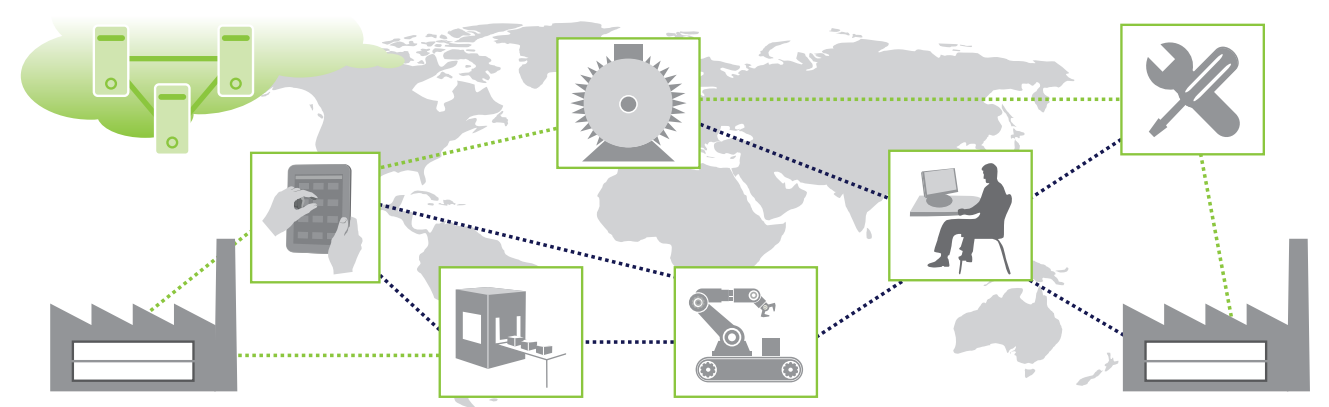
\includegraphics[width=0.5\linewidth]{Bilder/A3_HorizontaleIntegration}
	\caption{Schaubild horizontale Integration [12, BMBF, S.35]}
	\label{fig:HorizontaleIntegration}
\end{figure}

\noindent Die \textbf{vertikale Integration} (Abbildung \ref{fig:VertikaleIntegration}) in der Produktions- und Automatisierungstechnik und der IT erfordert "die Integration der verschiedenen IT-Systeme auf den unterschiedlichen Hierarchieebenen (beispielsweise die Aktor- und Sensorebene, Steuerungsebene, Produktionsleitebene, Manufacturing and Execution-Ebene, Unternehmensplanungsebene)" [12, BMBF, S.24] um eine durchgängige Lösung zu ermöglichen [12, BMBF, S.24].

\begin{figure}[h]
	\centering
	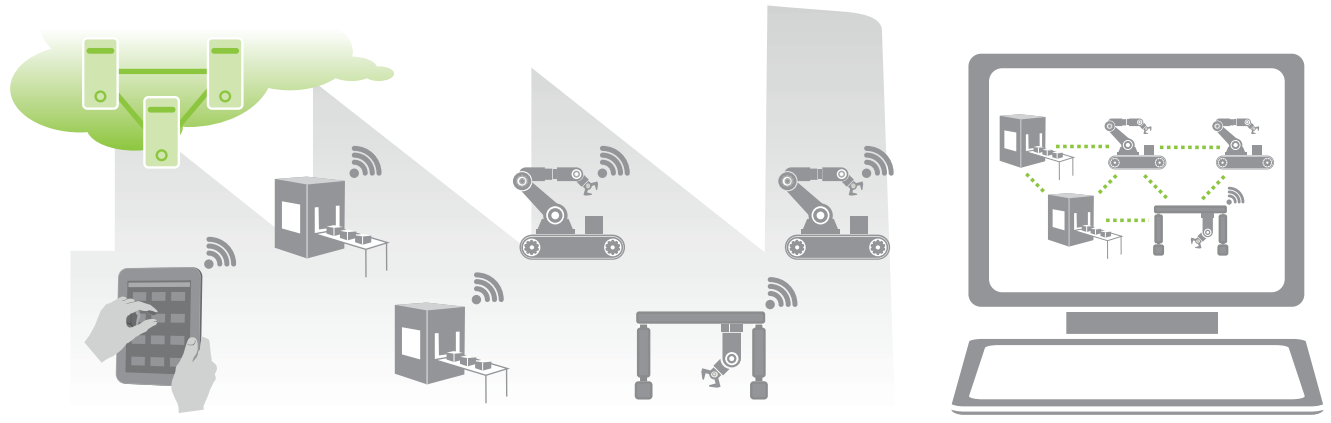
\includegraphics[width=0.5\linewidth]{Bilder/A4_VertikaleIntegration}
	\caption{Schaubild vertikale Integration [12, BMBF, S.36]}
	\label{fig:VertikaleIntegration}
\end{figure}

\subsubsection{Souveränität}\label{sec:Souveränität}

Souveränität soll die „Freiheit alles Akteure am Markt selbstbestimmte, unabhängige Entscheidungen zu treffen“ [3, Plattf.I, S.4] und einen Fairen Wettbewerbs ermöglichen [3, Plattf.I, S.4]. Souveränität erfordert:
\begin{enumerate}
	\item \textbf{Digitale Infrastruktur} [3, Plattf.I, S.4] \\
	Es wird eine über Unternehmensgrenzen hinweg reichende leistungsstarke und souveräne
	Infrastruktur benötigt. „Diese Infrastruktur muss für alle Teilnehmer gleichermaßen offen 
	zugänglich sein und ohne Einschränkungen zur Verfügung stehen“ [3, Plattf.I, S.4].
	\item \textbf{Sicherheit} [3, Plattf.I, S.4] \\
	„Datenschutz, IT- und Informationssicherheit stellen einen fest etablierten industriellen
	und gesellschaftlichen Wert dar“ [3, Plattf.I, S.4] und sind somit „eine Grundvoraussetzung
	für Industrie 4.0 und die Kooperation innerhalb digitaler Ökosysteme“ [3, Plattf.I, S.4].
	\item \textbf{Technologieentwicklung} [3, Plattf.I, S.4] \\
	Der Fortschritt von Industrie 4.0 basiert auf „Forschung, Entwicklung und Innovationen“ 
	[3, Plattf.I, S.4], daher sollen alle Teilnehmer am Wettbewerb „an den technologischen 
	Entwicklungen partizipieren und profitieren“ [3, Plattf.I, S.4].
\end{enumerate}

\subsubsection{Interoperabilität}\label{sec:Interoperabilität}
Ein zentraler Bestandteil der Industrie 4.0 ist die „flexible Vernetzung unterschiedlicher Akteure“ [3, Plattf.I, S.5]. Um eine Vernetzung zwischen vielen verschieden Akteuren zu gewährleisten ist die Interoperabilität eine Schlüsselkomponente. Es wird vorausgesetzt, dass alle Teilnehmer sich an die Standards zur Interoperabilität einhalten, aktiv zu der Entwicklung dieser Standards beitragen und somit eine „Vernetzung über Unternehmens- und Branchengrenzen hinweg“ [3, Plattf.I, S.5] ermöglichen [3, Plattf.I, S.5]. Interoperabilität erfordert:
\begin{enumerate}
	\item \textbf{Standards und Integration} [3, Plattf.I, S.5] \\
	Standards und stellen die Basis für die Interoperabilität dar und erleichtern die Integration
	von neunen Komponenten. Das Entwickeln von branchenübergreifenden Standards und
	Referenzarchitekturen ist aufwendig [3, Plattf.I, S.5].
	\item \textbf{Regulatorischer Rahmen} [3, Plattf.I, S.5] \\
	Ein regulatorischer Rahmen ist notwendig, um „faire und gleiche Bedingungen für alle
	Akteure sicherzustellen“ [3, Plattf.I, S.5].
	\item \textbf{Dezentrale Systeme und Künstliche Intelligenz} [3, Plattf.I, S.5] \\
	Dezentrale Systeme und Künstliche Intelligenz sind für die industrielle Wertschöpfung im 
	B2B-Bereich von wesentlich größerer Bedeutung als im B2C-Bereich. Die Nutzung,
	Verknüpfung und Auswertung von Maschinen- und Nutzerdaten erfordert ein gut vernetztes
	Ökosystem. Um Künstliche Intelligenz sinnvoll einsetzen zu können, muss „die Gewinnung 
	und Nutzung von Smart Data“ [3, Plattf.I, S.5] ermöglicht werden. Smart Data sind Daten, die 
	von intelligenten Produkten mit integrierten Chips über die gesamte Lebensdauer des 
	Produktes gesammelt werden.
\end{enumerate}

\subsubsection{Nachhaltigkeit}\label{sec:Nachhaltigkeit}
Nachhaltigkeit ist von zentraler Bedeutung für den Wandel zu Industrie 4.0, denn „ökonomische, ökologische und soziale Nachhaltigkeit stellen einen fundamentalen Eckpfeiler der gesellschaftlichen Wertorientierung dar“ [3, Plattf.I, S.6]. Des Weiteren trägt die Nachhaltigkeit „entscheidend zur Erhaltung des Lebensstandards der Gesellschaft bei“ [3, Plattf.I, S.6]. Nachhaltigkeit erfordert:
\begin{enumerate}
	\item \textbf{Gute Arbeit und Bildung} [3, Plattf.I, S.6] \\
	Um ein hohes Beschäftigungsniveau zu halten und wettbewerbsfähig zu bleiben, müssen
	Weiterbildungsmöglichkeiten geschaffen werden [3, Plattf.I, S.6].
	\item \textbf{Gesellschaftliche Teilhabe} [3, Plattf.I, S.6] \\
	Da Industrie 4.0 „einen gesamtgesellschaftlichen Transformationsprozess“ [3, Plattf.I, S.6]
	darstellt, erfordert der Wandel die Beteiligung und Mitbestimmung aller Akteure [3, Plattf.I, 
	S.6].
	\item \textbf{Klimaschutz} [3, Plattf.I, S.6] \\
	Um den Klimaschutz zu gewährleisten bedarf es einer steigenden Ressourceneffizienz
	und einem besseren Recycling von Stoffen [3, Plattf.I, S.6].
\end{enumerate}

\subsection{Leitfaden für Industrie 4.0}\label{sec:LeitfadenUmsetung}
Da es wie bereits erwähnt keinen allgemein anwendbaren Lösungsweg gibt, haben einige Organisationen einen Leitfaden für den Wandel zu Industrie 4.0 angefertigt. Im Folgenden wird der Leitfaden „Leitfaden Industrie 4.0 – Orientierungshilfe zur Einführung in den Mittelstand“ vom Verband Deutscher Maschinen- und Anlagebauer (VDMA) vorgestellt.
\newline
Der Leitfaden soll mittelständischen Unternehmen einen Werkzeugkasten bieten, der Ihnen bei der Entwicklung „eigenständiger Industrie 4.0 Geschäftsmodelle“ [2, VDMA, leit, S.6] behilflich ist. Des Weiteren soll der Leitfaden keine allgemeingültige Strategie darstellen, sondern die Unternehmen dabei unterstützen ihre eigenen Stärken und Kompetenzen bei ihrer Weiterentwicklung zu berücksichtigen [2, VDMA, Leitfaden, S.6]. Wie in Abbildung \ref{fig:VDMAAufbauLeitfaden} zu sehen ist, umfasst der Leitfaden insgesamt fünf Phasen: Vorbereitungs-, Analyse-, Kreativitäts-, Bewertungs- und Einführungsphase [2, VDMA, Leitfaden, S.6].
\begin{figure}[h]
	\centering
	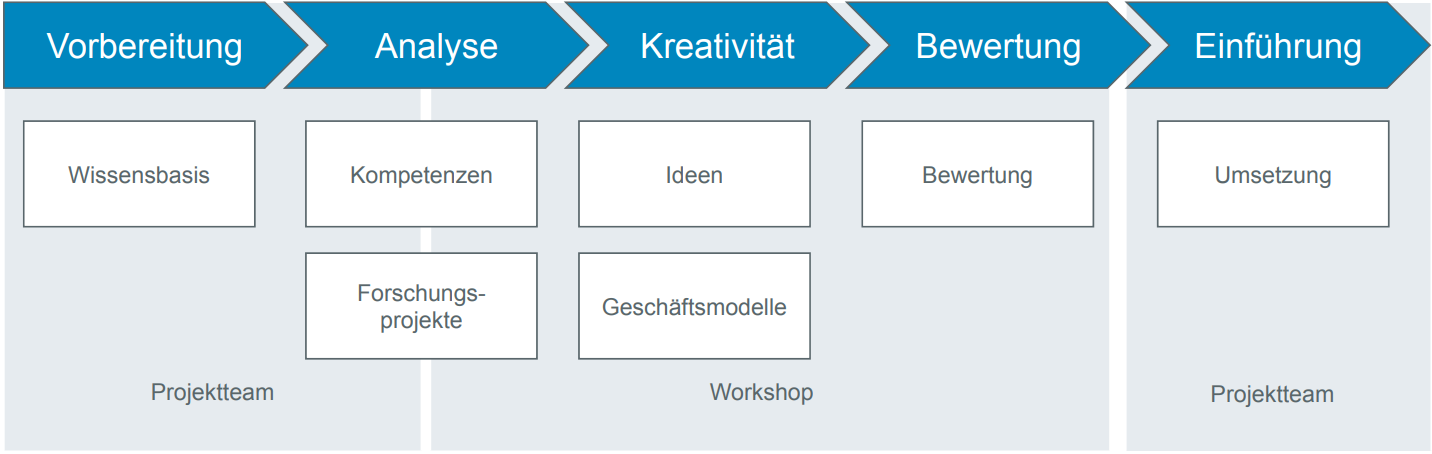
\includegraphics[width=1\linewidth]{Bilder/A5_VDMA_Phasen}
	\caption{VDMA - Aufbau des Leitfadens [2, VDMA, S.10]}
	\label{fig:VDMAAufbauLeitfaden}
\end{figure}
\begin{enumerate}
	\item \textbf{Vorbereitungsphase:} \\ In der ersten Phase soll eine Wissensbasis für alle Teilnehmer geschaffen werden. Das Unternehmen soll Kenntnisse über den Markt und über ihr eigenes Produkt aufbauen. Diese grundlegende Wissensbasis ist der „Ausgangspunkt für die Erarbeitung von Produktideen und Verbesserungen in der internen Produktion“ [2, VDMA, Leitfaden, S.10].
	\item \textbf{Analysephase:} \\ In der zweiten Phase werden die Kompetenzen des Unternehmen im Bereich von Industrie 4.0 Technologien untersucht. Die Kompetenzen des Unternehmens werden sowohl produktseitig als auch produktionsseitig untersucht. Diese Phase liefert eine „Ausgangsbasis für die spätere Ideengenerierung“ [2, VDMA, Leitfaden, S.10].
	\item \textbf{Kreativitätsphase:} \\ In der dritten Phase geht es um die „Generierung neuer Ideen und die anschließende Ausarbeitung von Konzepten für Geschäftsmodelle“, basierend auf dem aufgebauten Wissen der vorherigen zwei Phasen [2, VDMA, Leitfaden, S.10].
	\item \textbf{Bewertungsphase:} \\ In der vierten Phase werden die zuvor erarbeiteten Konzepte bewertet um Geschäftsmodelle „mit hohem Potential bei geringen Ressourceneinsatz“ [2, VDMA, Leitfaden, S.10].  zu identifizieren [2, VDMA, Leitfaden, S.10].
	\item \textbf{Einführungsphase:} \\ In der fünften und letzten Phase geht es um die Ausarbeitung der gesammelten Konzepte, damit diese „in entsprechende Projekte überführt und vorangetrieben“ [2, VDMA, Leitfaden, S.10] werden können.
\end{enumerate}
Zentrales Element des Leitfadens ist der sogenannte „Werkzeugkasten Industrie 4.0“, der in  Abbildung \ref{fig:VDMAWerkzeugkasten} zu sehen ist. Der Werkzeugkasten „zeigt Entwicklungsstufen für verschiedene Anwendungsebenen von Industrie 4.0 auf“ [2, VDMA, Leitfaden, S.11] und soll bei der „schrittweisen Umsetzung innovativer Ideen in kleinen und mittelständischen Unternehmen“ behilflich sein [2, VDMA, Leitfaden, S.11]. Dabei ist der Werkzeugkasten unterteilt in zwei Hälften: Produkte und Produktion. Die einzelnen Entwicklungsstufen auf jeder Anwendungsebene sind in steigender Komplexität von links nach rechts sortiert. Es ist anzumerken, dass der Werkzeugkasten weiterentwickelt werden muss, da „die Entwicklungen der vierte industrielle Revolution noch lange nicht abgeschlossen“ [2, VDMA, Leitfaden, S.11] sind und daher einige „technologische Entwicklungsstufen nicht umfänglich vorausgesagt werden können“ “ [2, VDMA, Leitfaden, S.11].
\begin{figure}[h]
	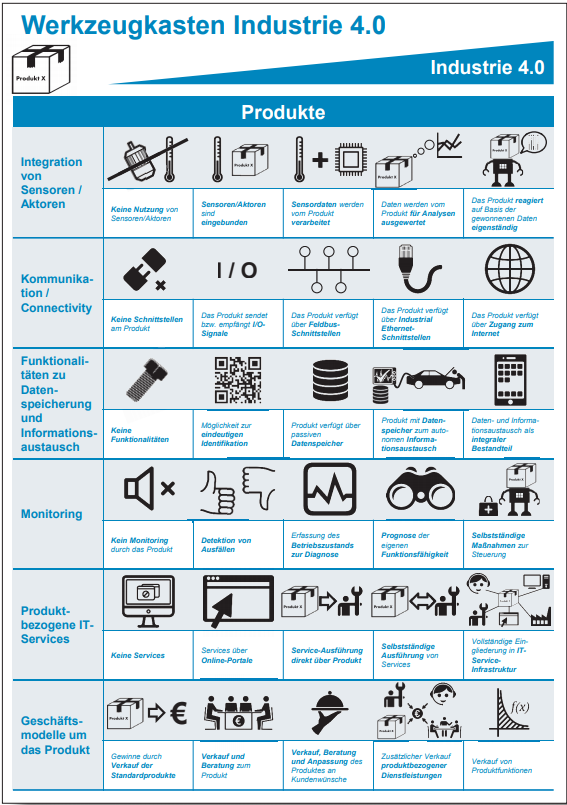
\includegraphics[width=0.5\linewidth]{Bilder/A6_VDMAWerkzeugkasten1}
	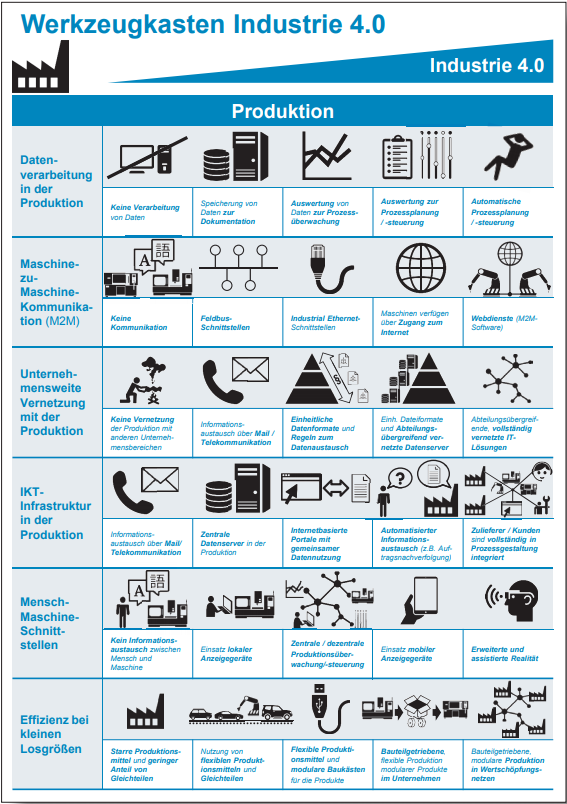
\includegraphics[width=0.5\linewidth]{Bilder/A7_VDMAWerkzeugkasten2}
	\caption{VDMA - Werkzeugkasten Industrie 4.0 [2, VDMA, S.9]}
	\label{fig:VDMAWerkzeugkasten}
\end{figure}
\\ Der Bereich der Produkte befasst sich mit der Frage, inwiefern sich mit Hilfe von Industrie 4.0 Produkte entwickeln (oder auch weiterentwickeln) lassen können, sodass diese für Kunden einen Mehrwert liefern. Auf der Seite der Produkte umfasst der Werkzeugkasten folgende Anwendungsebenen [2, VDMA, Leitfaden, S.13]:
\begin{enumerate}
	\item \textbf{Integration von Sensoren und Aktoren:} \\ Die Entwicklungen auf dieser Anwendungsebene reichen von Produkten mit keinen Sensoren/Aktoren, bis hin zu Produkten die auf Basis der gewonnen Daten eigenständig reagieren und mit den Cyber-Physischen-Systemen kommunizieren können [2, VDMA, Leitfaden, S.13].
	\item \textbf{Kommunikation und Konnektivität:} \\ Die Entwicklungen auf dieser Anwendungsebene reichen von Produkten die keine Schnittstelle zur Außenwelt besitzen, bis hin zu Produkten die über eine Anbindung zum Internet verfügen [2, VDMA, Leitfaden, S.13].
	\item \textbf{Funktionalitäten zur Datenspeicherung und dem Informationsaustausch:} \\ Die Entwicklungen auf dieser Anwendungsebene reichen von Produkten die keine Funktionalitäten zur Datenspeicherung und Informationsaustausch besitzen, bis hin zu Produkten bei denen dies ein integraler Bestandteil ist [2, VDMA, Leitfaden, S.13].
	\item \textbf{Monitoring:} \\ Die Entwicklungen auf dieser Anwendungsebene reichen von Produkten die kein eigenständiges Monitoring durchführen können, bis hin zu Produkten die selbstständig Maßnahmen zur Steuerung der Produktion übernehmen können [2, VDMA, Leitfaden, S.13].
	\item \textbf{Produktbezogene IT-Services:} \\ Die Entwicklungen auf dieser Anwendungsebene reichen von Produkten die keine zusätzlichen Dienstleistungen anbieten, bis hin zu Produkten die vollständig eingegliedert sind in eine übergeordnete IT-Service-Infrastruktur [2, VDMA, Leitfaden, S.13].
	\item \textbf{Geschäftsmodelle um das Produkt:} \\ Die Entwicklungen auf dieser Anwendungsebene reichen von Produkte bei denen der Gewinn nur durch den Verkauf der Produkte gemacht wird, bis hin zu Produkten bei denen Gewinn durch den Verkauf zusätzlicher Produktfunktionen (z.B. Dienstleistungen) gesteigert wird [2, VDMA, Leitfaden, S.13].
\end{enumerate}
Im Bereich der Produktion beschäftigt man sich mit der Frage, wie Industrie 4.0 den Unternehmen es ermöglichen kann, dass sowohl Produktionsabläufe optimiert als auch Produktionskosten gesenkt werden. Auf der Seite der Produktion umfasst der Werkzeugkasten folgende Anwendungsebenen [2, VDMA, Leitfaden, S.15]:
\begin{enumerate}
	\item \textbf{Datenverarbeitung} \\ in der Produktion: Die Entwicklungen auf dieser Anwendungsebene reichen von Produktionsanlagen die keine Daten verarbeiten, bis hin zu Produktionsanlagen mit automatisierten Prozessplanungen und Steuerungen.
	\item \textbf{Maschine-zu-Maschine-Kommunikation (M2M):} \\ Die Entwicklungen auf dieser Anwendungsebene reichen von Produktionsanlagen die keine Form von Kommunikation zwischen Maschinen ermöglichen, bis hin zu Produktionsanlagen die durch eine Internet-Schnittstelle eingebunden sind in Webdienste (Cloud).
	\item \textbf{Unternehmensweite Vernetzung mit der Produktion:} \\ Die Entwicklungen auf dieser Anwendungsebene reichen von Produktionsanlagen bei denen die Produktion nicht mit anderen Unternehmensbereichen vernetzt ist, bis hin zu Unternehmen die eine Abteilungsübergreifende vernetzte IT-Infrastruktur besitzen.
	\item \textbf{IKT-Infrastruktur in der Produktion:} \\ Die Entwicklungen auf dieser Anwendungsebene reichen von Produktionsanlagen bei denen der gesamte Informationsaustausch über Mail oder Telekommunikation stattfindet, bis hin zu Unternehmen bei denen die Zulieferer/Kunden vollständig in der Prozessgestaltung integriert sind.
	\item \textbf{Mensch-Maschine-Schnittstellen:} \\ Die Entwicklungen auf dieser Anwendungsebene reichen von Produktionsanlagen deren Maschinen keinen direkten Informationsaustausch mit den Menschen ermöglichen, bis hin zu Produktionsanlagen bei denen die Mitarbeiter mit Hilfe von Erweitertet und Assistierter Realität direkt Informationen von den Maschinen auslesen können.
	\item \textbf{Effizient bei kleinen Losgrößen:} \\ Die Entwicklungen auf dieser Anwendungsebene reichen von Produktionsanlagen die nicht dynamisch und somit ineffizient bei kleinen Losgrößen sind, bis hin zu bauteilgetriebenen modularen Produktionen, ermöglicht durch Wertschöpfungsnetze.
\end{enumerate}
Für diese Arbeit ist die Anwendungsebene „Mensch-Maschine-Schnittstelle“ auf der Produktionsseite des Werkzeugkastens am relevantesten, da der Einsatz von erweiterter Realität (Virtual Reality) die Kommunikation zwischen Mensch und Maschine maßgeblich verändert. Diese Entwicklung ermöglicht einige neue Geschäftsmodelle im Bereich von Industrie 4.0, wie z.B. die standortunabhängige Interaktion mit Produktionsanlagen mit Hilfe von Virtual Reality Brillen.

%--------------------------------------------------------------------------------------------------
\section{Die Ausgangslage der industriellen Fertigung}\label{sec:IndustrielleFertigung}

In diesem Kapitel gibt es einen Einblick in den Produktlebenszyklus und die Automatisierungspyramide der industriellen Fertigung.

%Damit alle zitate generiert werden, nur vorläufig
\cite{2}
\cite{3}
\cite{4}
%\cite{5}
%\cite{6}
%\cite{7}

\subsection{Der Produktlebenszyklus}\label{sec:Produktlebenszyklus}

\subsection{Die Automatisierungspyramide}\label{Automatisierungspyramide}

%--------------------------------------------------------------------------------------------------
%\section{Mensch-Computer Interaktion}\label{sec:HCI}

%\lipsum[2]

%\subsection{Die Geschichte der Mensch-Computer Interaktion}\label{sec:HCIGeschichte}

%\lipsum[2]

%\subsection{Relevanz für meine Arbeit}\label{sec:RelevanzHCI}

%\lipsum[2]

%\subsection{???}\label{sec:???}

%\lipsum[2]

%--------------------------------------------------------------------------------------------------
%\section{Virtual Reality}\label{sec:VR}

%\lipsum[2]

%\subsection{Die Geschichte von Virtual Reality Hardware}\label{sec:VRGeschichte}

%\lipsum[2]

%\subsection{Stand der Technik}\label{sec:VRStandDerTechnik}

%\lipsum[2]

%\subsection{Technische Herausforderungen}\label{sec:VRHerausforderungen}

%\lipsum[2]

%\subsection{Potential und Ausblick}\label{sec:VRPotentialUndAusblick}

%\lipsum[2]

%\subsection{????}\label{sec:????}

%\lipsum[2]

%--------------------------------------------------------------------------------------------------